\newpage

\chapter{Equivariant Priors for Compressed Sensing} 
\newpage
%%%%%%%%%%%%%%%%%%%%
%Group Convolutional Neural Network
%%%%%%%%%%%%%%%%%%%%
\section[Group Theory and Equivariant Neural Networks]{Group Theory and \\ Equivariant Neural Networks}

We review some basics of group theory and group convolutional neural networks. There are other ways of building equivariant networks beyond group convolutional neural networks, see for example \cite{e2cnn,cohen_steerable_2016,Kondor2018-GENERAL,cesa2022a}. Our theoretical results and equivariant VAE constructions are oblivious to the choice of architecture. 

For a set $\gG$, a law of composition $\cdot : \gG \times \gG \to \gG$ is a mapping that maps $h, g\in\gG$ to $h \cdot g\in\gG$. A \textit{group} is a set $\gG$ with a  law of composition $\cdot : \gG \times \gG \to \gG$, called {group law},  which satisfies following properties:
    \begin{itemize}
        \item The law $\cdot$ is associative: $a \cdot (b \cdot c) = (a \cdot b) \cdot c$ for all $ a, b, c \in \gG$
        \item There is an identity element in $\gG$, denoted by $1$, such that $a \cdot 1 = 1 \cdot a = a$ for all $a\in\gG$
        \item Every element of $a\in\gG$ has an inverse, denoted by $b$ such that $a\cdot b=1$ and $b\cdot a=1$.
    \end{itemize}

A group $\gG$ is an abelian group if the group law is {commutative}, namely $a\cdot b =b \cdot a$. 
A group $\gG$ is {finite} if the set $\gG$ is finite. A group $\gG$ is a {compact} group if $\gG$ is a compact topological space with continuous group operation.

For an arbitrary space $\gX$, we can define the action of the group $\gG$ by a mapping $\gT_g: \gG \times \gX \to \gX$, which maps $\vx\in\gX$ and $g\in\gG$ to $\gT_g\vx$. For the identity element, $\vx$ is mapped to itself. In this work, the action of the group is assumed to be linear on a vector space $\gX$, and $\gT_g$ has a matrix representation. The action of the group $\gG$ satisfies group properties indicates above, and therefore, $\gT_g$ is a linear representation of the group $\gG$ on $\gX$. Representation theory characterizes linear representations of groups on general vector spaces. We work with unitary representations, that is,  $\gT_g$ is a unitary transformation.


A mapping $f:\gX\to\gY$ is equivariant to the action of the group $\gG$ if
\[
f(\gT^{\gX}_g\vx) =\gT^{\gY}_g f(\vx),
\]
where $\gT^{\gX}_g$ and $\gT^{\gY}_g$ are linear representations of the group $\gG$ on $\gX$ and $\gY$. 


%%%%%%%%%%%%%%%%%%%%%%%
\paragraph{Group Convolution} One example of equivariant neural networks is  group equivariant convolutional networks \cite{cohen2016group}. 
The group convolution is defined on the space $\gX$ as:
\begin{align}
    \forall g \in \gG \quad  (\vw \gconv \vx)(g) := \langle \gT_g\vw, \vx \rangle, 
\label{def:group_conv}
\end{align}
where $\vw,\vx\in\gX$. The group convolution is an equivariant transformation w.r.t. the actions of group $\gG$. Note that $(\vw \gconv \vx)\in\R^{|\gG|}$, and the actions of group $\gG$ on $\vx\in\R^{|\gG|}$ is permuting the entries of $\vx$. This means that the regular representation $\gG$ is used as group representation \cite{serre1977linear}. 

Each group convolution can be seen as a function defined on the group $\gG$, and therefore, after the first layer, we can focus on functions on $\gG$ determined by $|\gG|$-dimensional vectors. 
Given the group $\gG=(g_0, g_1, \dots, g_i, \dots, g_{|G|-1})$, and vectors $\vx, \vw \in \R^{|\gG|}$, the group convolution can be defined by a matrix multiplication between the vector $\vx$ and a matrix $\mW$:
\begin{equation}
    (\vw \gconv \vx)(g_i) = (\mW\vx)[i]
\end{equation}
where the matrix $\mW$ is given as follows:
\begin{equation}
    \mW=\begin{pmatrix}
    w(g_0)& \dots & w(g_{|\gG|-1})\\
    w(g_1^{-1}g_0) & \dots&   w(g_1^{-1}g_{|\gG|-1})\\
    \vdots &\ddots &\vdots \\
    w(g_{|\gG|-1}^{-1}g_0) & \dots&   w(g_{|\gG|-1}^{-1}g_{|\gG|-1}).\\
    \end{pmatrix}
\label{eq:group_circulant}
\end{equation}
A group convolutional neural network is defined by concatenating group convolution layers with pointwise non-linearities in the middle. At each layer, multiple 
kernel like $\vw$ can be chosen, each one corresponding to a single channel. It is possible to use other representations of the group $\gG$ to build equivariant networks (see \citet{cohen_steerable_2016,e2cnn} for some examples). 

% where the $i$-th entry contains the value of the function evaluated on $g_i$:
% \begin{equation}
%     \vx=
%     \begin{pmatrix}
%     x(g_0)\\
%     \vdots\\
%     x(g_{|G|-1})
%     \end{pmatrix},\quad 
%         \vw=
%     \begin{pmatrix}
%     w(g_0)\\
%     \vdots\\
%     w(g_{|G|-1})
%     \end{pmatrix}.
% \end{equation}
% The same holds for the output signal $w \gconv x$. Define matrix $\mW$ as follows:
% \begin{equation}
%     \mW=\begin{pmatrix}
%     w(g_0)& \dots & w(g_{|G|-1})\\
%     w(g_1^{-1}g_0) & \dots&   w(g_1^{-1}g_{|G|-1})\\
%     \vdots &\ddots &\vdots \\
%     w(g_{|G|-1}^{-1}g_0) & \dots&   w(g_{|G|-1}^{-1}g_{|G|-1})\\
%     \end{pmatrix}
% \label{eq:group_circulant}
% \end{equation}
% Then, the group convolution can then be expressed as a matrix multiplication between the vector $\vx$ and a matrix $\mW$ containing at position $(i, j)$ the entry of $w_{g_i^{-1} g_j}$:
% \begin{equation}
%     (w \gconv h.x)(g_i) = (\mW\vx)[i]
% \end{equation}
% The matrix $\mW$ contains permuted copies of its first row, where the respective permutation matrix is determined by group actions.
% Assuming $g_0 = e$ is the identity, the first row of $\mW$ contains $\vw^T$ while the $i$-th row contains $(g_i.\vw)^T$, i.e. the vector representing the signal $g_i.w$. The matrix $\mW$ is a $G$-\textbf{circulant matrix}.




% Given a space $\gX$ associated with the action of a group $G$ and an invariant inner product $\langle \cdot, \cdot \rangle: \gX \times \gX \to \R$, we define the \textit{group convolution} $w \gconv x : G \to \R$ of two elements $w, x \in \gX$ as
% \begin{align}
%     \forall g \in G \quad  (w \gconv x)(g) := \langle g.w, x \rangle \ .
% \label{def:group_conv}
% \end{align}
% % Note that what we defined is technically a \textbf{group cross-correlation} and so it differs from the usual definitions of convolution over groups.
% % We still refer to is as group convolution to follow the common terminology in the Deep Learning literature.
% Group convolution satisfies the following equality:
% \begin{align}
%     \label{eq:fourier_conv_theorem}
%     \widehat{w \gconv x}(\psi) &= \hat{x}(\psi) \hat{w}(\psi)^T
% \end{align}

% The classical definition of \textit{group convolution} between two signals $w, x : G \to \R$ is a special case of the one above in the case $\gX$ is the space of square integrable functions over $G$ and the invariant inner product is defined as:
% \begin{align*}
%     \langle w, x \rangle := \int_{g \in G} w(g) x(g) \ d\mu(g)
% \end{align*}
% where $\mu: G \to \R$ is a Haar measure over $G$.
% The group convolution, then, becomes 
% \[
%     (w \gconv x)(g) := \int_{h \in G} w(g^{-1} h) x(h) \ d\mu(h) =\int_{h \in G} w(h) x(g.h) \ d\mu(h) \ .
% \]
% Note that what we defined is technically a \textbf{group cross-correlation}, and so it differs from the usual definitions of convolution over groups.
% We still refer to is as group convolution to follow the common terminology in the deep learning literature. 

% When $G$ is finite, the Haar measure is the counting measure and the integral becomes a sum. Fix an ordering of group elements as  $(g_0, g_1, \dots, g_i, \dots, g_{|G|-1})$ with $g_0=e$ the identity element. The signals $x, w : G \to \R$ can be stored as $|G|$ dimensional vectors $\vx, \vw \in \R^{|G|}$, where the $i$-th entry contains the value of the function evaluated on $g_i$:
% \begin{equation}
%     \vx=
%     \begin{pmatrix}
%     x(g_0)\\
%     \vdots\\
%     x(g_{|G|-1})
%     \end{pmatrix},\quad 
%         \vw=
%     \begin{pmatrix}
%     w(g_0)\\
%     \vdots\\
%     w(g_{|G|-1})
%     \end{pmatrix}.
% \end{equation}
% The same holds for the output signal $w \gconv x$. Define matrix $\mW$ as follows:
% \begin{equation}
%     \mW=\begin{pmatrix}
%     w(g_0)& \dots & w(g_{|G|-1})\\
%     w(g_1^{-1}g_0) & \dots&   w(g_1^{-1}g_{|G|-1})\\
%     \vdots &\ddots &\vdots \\
%     w(g_{|G|-1}^{-1}g_0) & \dots&   w(g_{|G|-1}^{-1}g_{|G|-1})\\
%     \end{pmatrix}
% \label{eq:group_circulant}
% \end{equation}
% Then, the group convolution can then be expressed as a matrix multiplication between the vector $\vx$ and a matrix $\mW$ containing at position $(i, j)$ the entry of $w_{g_i^{-1} g_j}$:
% \begin{equation}
%     (w \gconv h.x)(g_i) = (\mW\vx)[i]
% \end{equation}
% The matrix $\mW$ contains permuted copies of its first row, where the respective permutation matrix is determined by group actions.
% Assuming $g_0 = e$ is the identity, the first row of $\mW$ contains $\vw^T$ while the $i$-th row contains $(g_i.\vw)^T$, i.e. the vector representing the signal $g_i.w$. The matrix $\mW$ is a $G$-\textbf{circulant matrix}.

%%%%%%%%%%%%%%%%%%%%
%Theory
%%%%%%%%%%%%%%%%%%%%
\newpage
\section[Recovery Guarantees  and Theoretical Analysis]{Recovery Guarantees  and \\ Theoretical Analysis} \label{appx:theory}
In this section, we present more details on theoretical guarantees for unknown rotation. We consider the following inverse problem with unknown rotation $g$: 
\begin{equation}
    \vy = \mA \gT_g^x \vx_\star + \vepsilon,
\end{equation}
where $\gT_g^x$ is the group representation in the input space. We work with unitary representations, which means that $(\gT_g^x)^{-1}=(\gT_g^x)^{H}$. We start by introducing some preliminary definitions.

\subsection{Definitions}
As we will see, we require the sensing matrix $\mA$ to satisfy certain constraints. The first on is set-restricted eigenvalue (S-REC) condition.
\begin{definition} A matrix $\mA$ is said to satisfy 
$\srec(\gS,\gamma,\delta)$ for some $\delta\geq 0$ and $\gamma>0$ and a set $\gS$ if for all $\vx,\vy\in\gS$:
\[
\norm{\mA(\vx-\vy)}_2\geq \gamma\norm{\vx-\vy}-\delta.
\]
\end{definition}
This is reminiscent of the null space property in compressed sensing. The idea is to guarantee that two points from the set of interest $S$ are \textit{separated} enough after mapping $\mA$, i.e., their difference lies away from the null space of $\mA$. 

The second condition on $\mA$ is that for every fixed $\vx\in\R^n$, we have:
\begin{equation}
    \norm{\mA\vx}_2\leq 2\norm{\vx}_2.
    \label{eq:norm_condition}
\end{equation}
Note that this bound needs to hold for a fixed $\vx$ and not all $\vx$, and therefore, this is a weaker assumption that bounding the spectral norm. We will see how these conditions are satisfied for a random Gaussian matrix.

% When the generative model $G(\cdot)$ is equivariant, we have: 
% \[
% \norm{G(z)-\gT_g^x \vx_\star}_2 = \norm{{\gT_g^x}^{H}G(z)- \vx_\star}_2 = \norm{G({\gT_g^z}^{H}z)- \vx_\star}_2
% \]


% As you can see in this theorem, the reconstruction error is upper bounded by $\min_{\vz}\norm{G(z)-\vx_\star}_2$.

% \begin{theorem}
% Consider an equivariant generative model $G: B_k(r)\to\R^n$, which is assumed to be an $L$-Lipschitz function. Let $\mA\in\R^{m\times n}$ be a random Gaussian matrix with i.i.d. entries $\gN(0,m^{-1})$. Assume that a signal $\vx^\star\in\R^n$ is observed in an unknown orientation according to $\vy = \mA \gT_g^x \vx + \vepsilon$. Suppose that $\hat{\vz}$ minimizes $\norm{\vy-\mA G(\vz)}$ to within error of $\delta_{\text{approx}}$.
% For measurement  number $m =\Omega(k \log (Lr/\delta)$, the following holds with probability $1-e^{-\Omega(m)}$
% \[
% \norm{G(\hat{\vz})-\gT_g^x \vx_\star}_2 \leq 6 \min_{\vz\in B_k(r)}\norm{G(\vz)-\vx_\star}_2 + 3\norm{\vepsilon}_2 + 2\delta_{\text{approx}} + 2\delta.
% \]
% \end{theorem}

% Note that the key point is the generative modeling with respect to canonical poses are relevant. 
% When the generative model is non-equivariant, even with known rotation, the problem 
% \[
% \norm{G(z)-\gT_g^x \vx_\star}_2 = \norm{{\gT_g^x}^{-1}G(z)- \vx_\star}_2
% \]
% Using equivariant generative priors, the recovery problem .
\subsection{Proof}
To train the generative prior, we assume that the data is given in a canonical orientation. The existence of a canonical orientation is not necessary. The following argument can be reworked by considering the quotient space and its proper parametrization instead. Without rotation, generative priors enjoy recovery guarantees of type provided in \citet{Bora2017-as}. For canonical orientations, the very same analysis holds for equivariant generative priors too.  The difference appears for the scenario with unknown orientation $g$. 

The proof for the equivariant priors follows standard steps exactly as \citet{Bora2017-as}. The reason is that unknown rotations are absorbed into the latent of the generative model so the main steps remain intact. We replicate the essence of the proof here to be self-contained.

The proof strategy for Theorem \ref{thm:equivmodel} is as follows. First, let $\hat{\vz}$ be the estimated latent that minimizes $\norm{\vy-\mA G(\vz)}$ to within error of $\delta_{\text{approx}}$. This means that for all $\vz$, we have
\[
\norm{\vy-\mA G(\hat{\vz})}_2\leq \norm{\vy-\mA G({\vz})}_2 +\delta_{\text{approx}}.
\]
Also, let $\vz_\star$ be the latent code\footnote{Existence of $\hat{\vz}$ and $\vz_\star$ follows from compactness of domain and continuity of the objective function. For a more general case, the proof can be replicated by replacing $\hat{\vz}$ and $\vz_\star$ with their definition.} minimizing $\norm{\vx_\star- G(\vz)}_2$. Note that the equivariance condition implies that:
\[
\gT_g^x G(\vz) =  G(\gT_g^z\vz),
\]
for group representation $\gT_g^x$ and $\gT_g^z$. Therefore, the unitary property of $\gT_g^x$ implies that 
\[
\norm{\vx_\star- G(\vz)}_2 = \norm{\gT_g^x\vx_\star- \gT_g^x G(\vz)}_2 = 
 \norm{\gT_g^x\vx_\star- G(\gT_g^z\vz)}_2.
\]
This means that $\gT_g^z\vz_\star$ is the minimizer of $ \norm{\gT_g^x\vx_\star- G(\vz)}_2$. According to the assumption of the theorem, and as seen above,  $\hat{\vz}$ and $\vz_\star$ satisfy:
\[
\norm{\vy-\mA G(\hat{\vz})}_2\leq \norm{\vy-\mA\gT_g^x G(\vz_\star)}_2+\delta_{approx}.
\]
The goal is to convert this inequality to another one in terms of $\norm{\gT_g^x\vx_\star- G(\hat{\vz})}_2$ and $\norm{\vx_\star-G(\vz_\star)}_2$. The main steps are contained in the following derivation:
\begin{align}
    \norm{\gT_g^x G(\vz_\star)- G(\hat{\vz})}_2&=
    \norm{ G(\gT_g^z\vz_\star)- G(\hat{\vz})}_2 \tag{equivariance}
    \\
    &\leq \frac{\norm{\mA G(\gT_g^z\vz_\star)-\mA G(\hat{\vz})}_2+ \delta}{\gamma}\tag{$\srec$}\\
    &\leq \frac{ 
    \norm{\vy-\mA G(\hat{\vz})}_2 
    +\norm{\vy-\mA \gT_g^x G(\vz_\star)}_2 + \delta
    }{\gamma}
    \tag{triangle ineq.}\\
    &\leq \frac{ 
    2\norm{\vy-\mA \gT_g^x G(\vz_\star)}_2 +\delta_{approx}+ \delta
    }{\gamma}
    \tag{theorem assumption}\\
    &\leq \frac{ 
    2\norm{\mA\gT_g^x\vx_\star-\mA \gT_g^x G(\vz_\star)}_2 +2\norm{\vepsilon}_2+\delta_{approx}+ \delta
    }{\gamma}
    \tag{triangle ineq.}\\
    &\leq \frac{ 
    4\norm{\gT_g^x\vx_\star- \gT_g^x G(\vz_\star)}_2 +2\norm{\vepsilon}_2+\delta_{approx}+ \delta
    }{\gamma}\tag{condition (\ref{eq:norm_condition})}
\end{align}
These inequalities, Lemma 4.3 in \citet{Bora2017-as}, only require triangle inequalities, $\srec$  property and bound on the condition (Eq.~\ref{eq:norm_condition}), where the last two conditions are satisfied by random Gaussian sensing matrices with i.i.d. entries and appropriately chosen variance. Using the following triangle inequality,
\begin{equation}
    \norm{\gT_g^x G(\vz_\star)- G(\hat{\vz})}_2\geq \norm{\gT_g^x\vx_\star- G(\hat{\vz})}_2 -\norm{\gT_g^x\vx_\star - \gT_g^x G(\vz_\star)}_2,
\end{equation}
and unitary property of $\gT_g^x$
\begin{equation}
\norm{\gT_g^x\vx_\star-\gT_g^x G(\vz_\star)}_2  = \norm{\vx_\star-  G(\vz_\star)}_2
\end{equation}
the theorem follows. 


Let's consider the $\srec$  property and the condition (Eq.~\ref{eq:norm_condition}). The later is satisfied by a random Gaussian matrix properly normalized. We use Gaussian concentration inequality to prove this.

\begin{theorem}[{Theorem 8.34  - \cite{foucart_mathematical_2013}}]
For a Lipschitz function $f:\R^n\to\R$ with Lipschitz constant $L$, if $\vg$ is a standard Gaussian random vector, then for all $t>0$, we have
\[
\mathbb{P}\left(f(\vg)-\E[f(\vg)]\geq t\right)\leq \exp\left(-\frac{t^2}{4L^2}\right).
\]
\end{theorem}
We choose $f$ as a function of the matrix $\mA$ and defined by $f(\mA)=\norm{\mA\vx}_2$. First, see that $f(\cdot)$ is Lipschitz with $L=\norm{\vx}_2$:
\[
\card{\norm{\mA\vx}_2 - \norm{\mB\vx}_2 }\leq \norm{\mA\vx-\mB\vx}_2\leq \norm{\mA-\mB}_2 \norm{\vx}_2\leq    \norm{\mA-\mB}_F \norm{\vx}_2.
\]
Therefore, we get, from the theorem, and for standard Gaussian random matrix $\mA$:
\[
\mathbb{P}(\norm{\mA\vx}_2-\E(\norm{\mA\vx}_2)\geq t)\leq \exp{\left(\frac{-t^2}{4\norm{\vx}^2_2}\right)}
\]
Note that $\E(f(\mA)=\E(\norm{\mA\vx}_2)$ can be upper bounded as: 
\[
\E(\norm{\mA\vx}_2)\leq (\E(\norm{\mA\vx}^2_2)^{1/2}=  (\sum_{i=1}^m \E(\inner{\va_i}{\vx})^2)^{1/2}  = (m\norm{\vx}^2_2)^{1/2}=\sqrt{m}\norm{\vx}_2.
\]
Finally, by choosing $t= \sqrt{m}\norm{\vx}_2$, we get with probability $1-e^{-m^2/4}$ that:
\[
\norm{\mA\vx}_2\leq t + \sqrt{m}\norm{\vx}_2 = 2 \sqrt{m}\norm{\vx}_2 
\]
Normalizing entries of the standard Gaussian random matrix $\mA$ by $1/\sqrt{m}$ will provide the desired result by choosing $\vx = \gT_g^x \vx^\star-\gT_g^x G(\vz_\star)$ which is a fixed vector independent of $\mA$.

The next step is, therefore, $\srec$ property. Since we use an equivariant generative model, the ambiguity about the rotation operation is captured in the latent space. Therefore, the very same approach of \citet{Bora2017-as} can be used to build $\epsilon$-nets and use that to establish $\srec$ for the equivariant generative model. We re-state this theorem for completeness here.

\begin{lemma}
For $L$-Lipshcitz equivariant generative model $G:\R^k\to\R^n$ and $\alpha<1$, the random Gaussian matrix $\mA\in\R^{m\times n}$ with i.i.d. entries $\gN(0,m^{-1})$ and $m =\Omega\left(\frac{k}{\alpha^2} \log (Lr/\delta)\right)$ satisfies $\srec(G(B_k(r)),1-\alpha,\delta)$ with probability $1-e^{-\Omega(\alpha^2m)}$.
\end{lemma}

Note that the proof of this lemma remains identical to \citet{Bora2017-as}, since the equivariance property does not play any role in the proof. It  is only necessary to establish it for a generative model $G$ and choosing $\gS=G(B_k(r))$.

% \gT_{g_\star}^x
% \gT_{\hat{g}}^x
As a final remark, consider for the moment the case of non-equivariant priors where the rotation needs to be extracted jointly with the latent code. In this case $\srec$ would translate to:
\begin{align}
    \norm{\gT_{g_\star}^x G(\vz_\star)- \gT_{\hat{g}}^x G(\hat{\vz})}_2&\leq 
 \frac{\norm{\mA \gT_{g_\star}^x G(\vz_\star)-\mA \gT_{\hat{g}}^x G(\hat{\vz})}_2+ \delta}{\gamma}.
\end{align}
In this case, we would need to establish $\srec$ for the set $\cup_{g\in\gG}\gT_{g}^x G(B_k(r))$. If the sets $\gT_{g}^x G(B_k(r))$ are disjoint for different $g$, the number of $\epsilon$-nets would increase, proportional to the $\epsilon$-net required to cover the group $\gG$. This would contribute another factor inside the logarithm for sample complexity.


% \begin{theorem}

% \end{theorem}

%%%%%%%%%%%%%%%%%%%%
%ADDITIONAL EXPERIMENTS
%%%%%%%%%%%%%%%%%%%%
\newpage
\section{Additional results} \label{appx:additional_exp}
% \subsection{VAE Priors}\label{appx:vae_conv_mlp}
% \begin{figure}[h]
%     \centering
%     \begin{tabular}{cc}
%         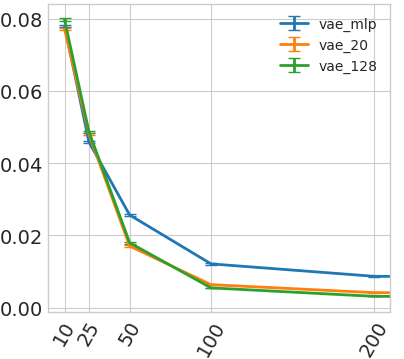
\includegraphics[width=0.4\textwidth]{new_images/vae_mse_no_rotation.png} &
%         \includegraphics[width=0.4\textwidth]{new_images/vae_mse_unknown_rotation copy.png} \\
%         \multicolumn{1}{c}{Number of measurements} &
%         \multicolumn{1}{c}{Number of measurements}\\
%     \end{tabular}
%     \caption{Comparison of MLP-VAE and Convolutional VAE with latent dimnetions 20 and 128 on MNIST dataset.}
%     \label{fig:vae_prior}
% \end{figure}
\subsection{Eq-VAE: group choice}\label{appx:eq_vae_group}

Group choice can be rather important to the performance of compressed sensing. Thus, we compare results of three different prior: equivariant under the cyclic group of $4$, $8$ and $16$ rotations. In Figure \ref{fig:vae_prior_group} we report MSE for CS on MNIST with 100 measurements. All three priors perform well, but the best results are achieved when we use the cyclic group of 16 rotations. 
\begin{figure}[h]
    \centering
    \begin{tabular}{cc}
        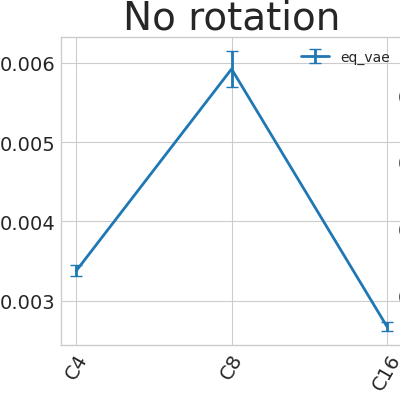
\includegraphics[width=0.4\textwidth]{pics/2_equiv_vae/eq_vae_group_no_rotation.png} &
        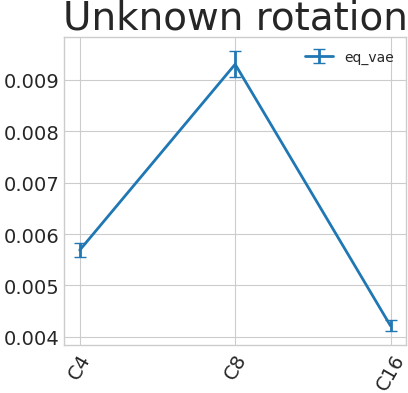
\includegraphics[width=0.4\textwidth]{pics/2_equiv_vae/eq_vae_group_rotation.png} \\
    \end{tabular}
    \caption{Compressed sensing with 100 measurements on MNIST. We compare VAE equivariant under the cyclic groups $C_4$, $C_8$ and $C_{16}$.}
    \label{fig:vae_prior_group}
\end{figure}

\newpage
\subsection{Eq-VAE: Samples}\label{appx:eq_vae_group_sample}
We report the compressed sensing results for the $C_{16}$-equivariant VAE. Figure~\ref{fig:vae_prior_samples} shows, how the reconstructions change when we apply the group action to a latent code and push it through the decoder (for three different latent codes). This way we observe that even though the model was not trained on the rotated images, it can generate them perfectly well.
\begin{figure}[h]
    \centering
    \begin{tabular}{cc}
        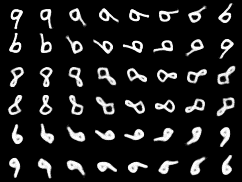
\includegraphics[width=0.8\textwidth]{pics/2_equiv_vae/mnist_reconstruction_full_covariance_non-cs.png} 
    \end{tabular}
    \caption{Samples from the equivariant VAE.}
    \label{fig:vae_prior_samples}
\end{figure}


\newpage
\subsection{Eq-VAE Priors for MAYO}\label{appx:eq_vae}

\begin{figure}[ht!]
    \centering
    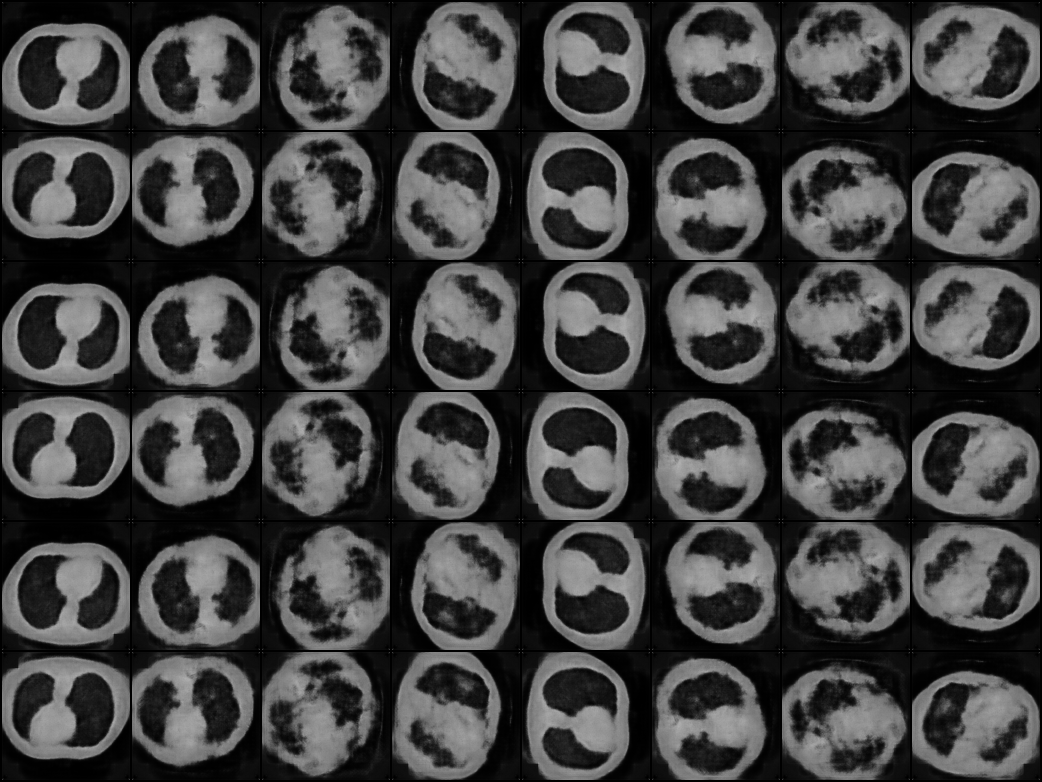
\includegraphics[width=0.5\textwidth]{pics/2_equiv_vae/mayo_rotated_reconstructed.png}
    \caption{
    Rotated reconstructions from Eq-VAEs for MAYO dataset.}
    \label{fig:mayo_train_points}
    \vspace*{\baselineskip}
\end{figure}
\begin{figure}[ht!]
    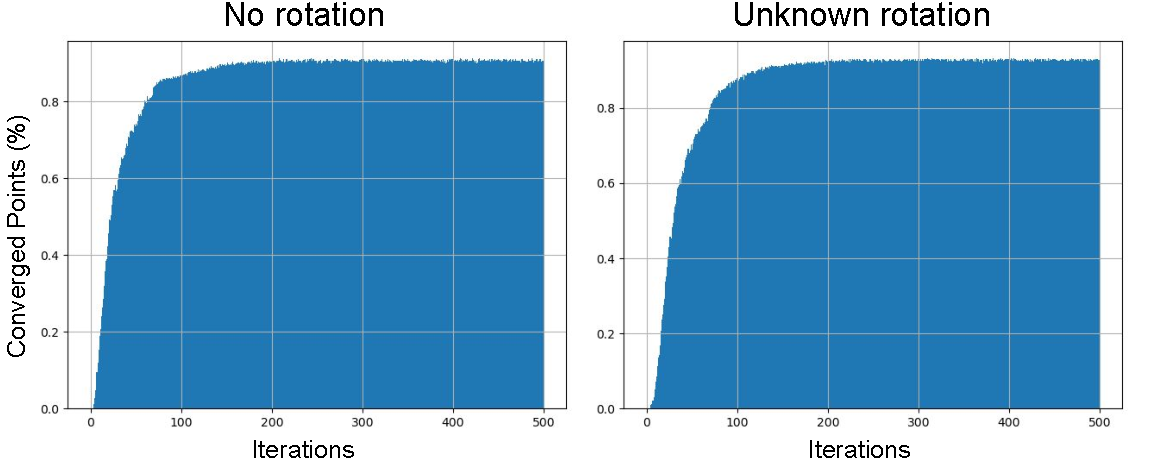
\includegraphics[width=\textwidth]{pics/2_equiv_vae/eqvae_iters_conv.pdf}\hfill
    \caption[][\baselineskip]{Number of iterations until convergence (i.e., MSE $\leq 1.e^{-2}$), for the MAYO dataset, using Eq-VAE as a generative prior. Left: No rotation angle. Right: Unknown rotations.}
    \label{fig:mayo_cdf_mse_conv}
    \vspace*{\baselineskip}
\end{figure}
\begin{figure}[ht!]
    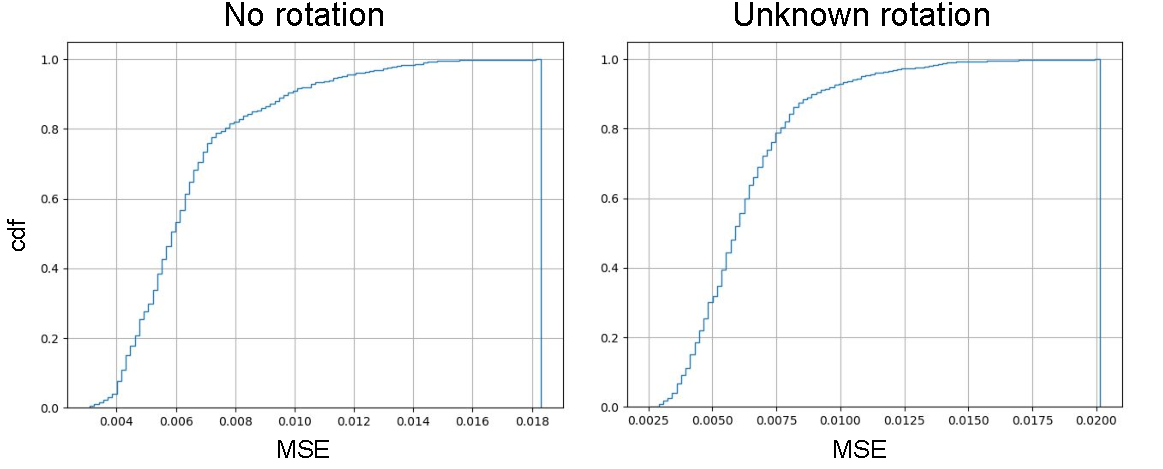
\includegraphics[width=\textwidth]{pics/2_equiv_vae/eqvae_mse.pdf}\hfill
    \caption[][\baselineskip]{MSE from compressed sensing experiments, for the MAYO dataset, using Eq-VAE as a generative prior. Left: No rotation angle. Right: Unknown rotations.}
    \label{fig:mayo_cdf_mse_eqvae}
    \vspace*{\baselineskip}
\end{figure}
\begin{figure}[ht!]
    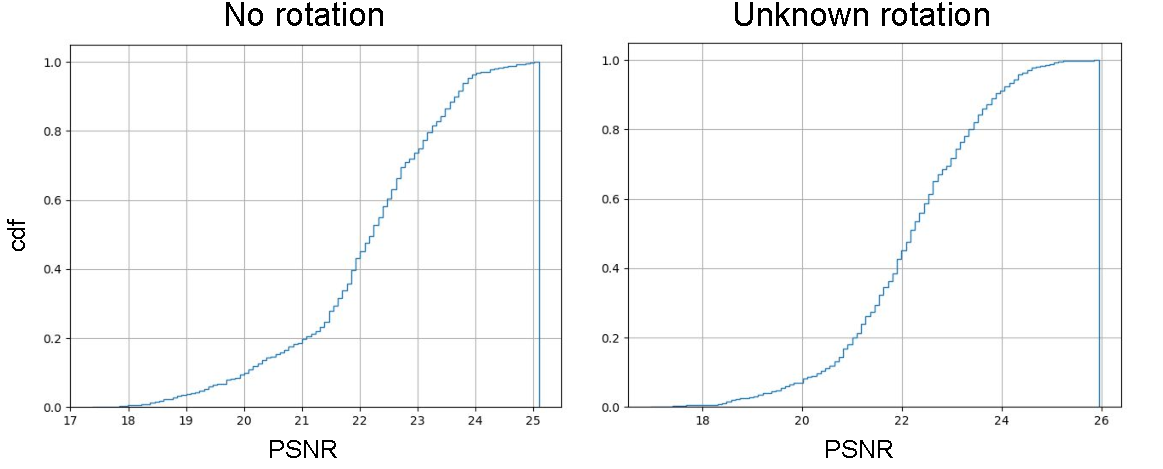
\includegraphics[width=\textwidth]{pics/2_equiv_vae/eqvae_psnr.pdf}
    \caption[][\baselineskip]{PSNR from compressed sensing experiments, for the MAYO dataset, using Eq-VAE as a generative prior. Left: No rotation angle. Right: Unknown rotations.}
    \label{fig:mayo_psnr}
       \vspace*{\baselineskip}
\end{figure}

%%%%%%%%%%%%%%%%%%%%
%Experimental details
%%%%%%%%%%%%%%%%%%%%
\newpage
\section{Experimental Setup}\label{appx:exp_setup}

% \subsection{Training Generative Prior}
\subsection{Training Convolutional VAE and Equivariant VAE}

\paragraph{Architecture} We train a VAE model, where both encoder and decoder are fully convolutional neural networks with the ReLU activations. 
% In Tables \ref{tab:mnist_arch} we report the exact architecture used for MNIST and MAYO dataset.

The representation space size is set to $z_{dim} = 128$. 

For MNIST, the Conv-VAE encoder is fully convolutional architecture with kernel size, number of filters, stride, and padding as follows: $\text{Input signal (1)} \rightarrow [(3, 32, 2, 1) \rightarrow (3, 64, 2, 1) \rightarrow (3, 96, 2, 1) \rightarrow (3, 128, 2, 1) \rightarrow (3, 256, 2, 1) \rightarrow flatten(.) \rightarrow (\mu_z, \log\sigma_z^2)]$. The decoder comprises of transpose convolutional layers. Following the preceding format, the architectural details of decoder is as follows: $\text{Input signal (128)} \rightarrow [(3, 128, 1, 0) \rightarrow (3, 96, 1, 0) \rightarrow (3, 64, 1, 1) \rightarrow (4, 32, 2, 1) \rightarrow (4, 1, 2, 1) \rightarrow flatten(.) \rightarrow (\mu_x)]$.

For MAYO, the Conv-VAE encoder is fully convolutional architecture with kernel size, number of filters, stride, and padding as follows: $\text{Input signal (1)} \rightarrow [(5, 32, 1, 0) \rightarrow (3, 32, 1, 0) \rightarrow (3, 64, 2, 0) \rightarrow (3, 64, 1, 0) \rightarrow (3, 128, 2, 0) \rightarrow (3, 128, 2, 0) \rightarrow (3, 256, 2, 0) \rightarrow (3, 256, 2, 0) \rightarrow (2, 256, 2, 0) \rightarrow flatten(.) \rightarrow (\mu_z, \log\sigma_z^2)]$. The decoder comprises of transpose convolutional layers. Following the preceding format, the architectural details of decoder is as follows: $\text{Input signal (128)} \rightarrow [(6, 256, 1, 0) \rightarrow (3, 256, 2, 0) \rightarrow (3, 128, 2, 0) \rightarrow (4, 128, 1, 0) \rightarrow (3, 64, 2, 0) \rightarrow (3, 32, 2, 0) \rightarrow (4, 32, 1, 0) \rightarrow (3, 1, 1, 0) \rightarrow flatten(.) \rightarrow (\mu_x)]$.

For MAYO, the Equivariant VAE encoder comprises of group equivariant convolutional architecture with kernel size, number of filters, stride, and padding as follows: $\text{Input signal (1)} \rightarrow [(5, 16, 1, 0) \rightarrow (3, 16, 1, 0) \rightarrow (3, 16, 2, 0) \rightarrow (3, 16, 2, 0) \rightarrow (3, 32, 2, 0) \rightarrow (3, 32, 1, 0) \rightarrow (3, 32, 1, 0) \rightarrow (3, 64, 1, 0) \rightarrow (2, 256, 2, 0)  \rightarrow flatten(.) \rightarrow (\mu_z, \log\sigma_z^2)]$. The decoder comprises of equivariant transpose convolutional layers. Following the preceding format, the architectural details of decoder is as follows: $\text{Input signal (128)} \rightarrow [(6, 128, 1, 0) \rightarrow (3, 32, 2, 0) \rightarrow (3, 128, 2, 0) \rightarrow (4, 32, 1, 0) \rightarrow (3, 16, 2, 0) \rightarrow (3, 16, 2, 0) \rightarrow (4, 8, 1, 0) \rightarrow (3, 8, 1, 0) \rightarrow (3, 1, 1, 0) \rightarrow flatten(.) \rightarrow (\mu_x)]$.

Note: Aug-VAE and Aug-Flow follow the same architecture as Conv-VAE and Flow respectively. The only difference between augmented and their non-augmented counterpart is that the augmented models are trained on augmented (rotated) dataset.

% \begin{table}[h]
% \caption{Architecture of convolutional VAE (latent dimension $=128$) deployed for MNIST dataset.}
% \label{tab:mnist_arch}
% \begin{center}
% \begin{tabular}{@{}lll@{}}
% \toprule
%                   & Encoder & Decoder  \\  \midrule
% & \texttt{Conv(3x3, 1->32, s=2, p=1)} & \texttt{ConvTranspose(3x3, 128->128, s=1, p=0, d=2)} \\
% & \texttt{ReLU()}& \texttt{ReLU()} \\
% & \texttt{Conv(3x3, 32->64, s=2, p=1)} & \texttt{ConvTranspose(3x3, 128->96, s=1, p=0)}\\
% & \texttt{ReLU()} & \texttt{ReLU()}\\
% & \texttt{Conv(3x3, 64->96, s=2, p=1)} &\texttt{ConvTranspose(3x3, 96->64, s=1, p=1)} \\
% & \texttt{ReLU()} &  \texttt{ReLU()} \\
% & \texttt{Conv(3x3, 96->128, s=2, p=1)} & \texttt{ConvTranspose(4x4, 64->32, s=2, p=1)} \\
% & \texttt{ReLU()} & \texttt{ReLU()} \\
% & \texttt{Conv(3x3, 128->128, s=2, p=1)} &  \texttt{ConvTranspose(4x4, 32->1, s=2, p=1)} \\
% & $\mu_z \leftarrow$ \texttt{Flatten()} & - \\
% & \texttt{Conv(3x3, 128->128, s=2, p=1)}&  $\mu_x \leftarrow$  \texttt{Sigmoid()} \\
% & $\log \sigma^2_z \leftarrow$ \texttt{Flatten()} & - \\
% \bottomrule
% \end{tabular}
% \end{center}
% \end{table}

% \begin{table}[h]
% \caption{Architecture of convolutional VAE (latent dimension $=128$) deployed for MAYO dataset.}
% \label{tab:mayo_arch}
% \begin{center}
% \begin{tabular}{@{}lll@{}}
% \toprule
%                   & Encoder & Decoder  \\  \midrule
% & \texttt{Conv(5x5, 1->32, s=1, p=0)} & \texttt{ConvTranspose(6x6, 128->256, s=1, p=0)} \\
% & \texttt{ReLU()}& \texttt{ReLU()} \\
% & \texttt{Conv(3x3, 32->32, s=1, p=0)} & \texttt{ConvTranspose(3x3, 256->256, s=2, p=0)}\\
% & \texttt{ReLU()} & \texttt{ReLU()}\\
% & \texttt{Conv(3x3, 32->64, s=2, p=0)} &\texttt{ConvTranspose(3x3, 256->128, s=2, p=0)} \\
% & \texttt{ReLU()} &  \texttt{ReLU()} \\
% & \texttt{Conv(3x3, 64->64, s=1, p=0)} & \texttt{ConvTranspose(4x4, 128->128, s=1, p=0)} \\
% & \texttt{ReLU()} & \texttt{ReLU()} \\
% & \texttt{Conv(3x3, 64->128, s=2, p=0)} & \texttt{ConvTranspose(3x3, 128->64, s=2, p=0)} \\
% & \texttt{ReLU()} & \texttt{ReLU()} \\
% & \texttt{Conv(3x3, 128->128, s=2, p=0)} & \texttt{ConvTranspose(3x3, 64->32, s=2, p=0)} \\
% & \texttt{ReLU()} & \texttt{ReLU()} \\
% & \texttt{Conv(3x3, 128->256, s=2, p=0)} & \texttt{ConvTranspose(4x4, 32->32, s=1, p=0)} \\
% & \texttt{ReLU()} & \texttt{ReLU()} \\
% & \texttt{Conv(3x3, 256->256, s=2, p=0)} & - \\
% & \texttt{ReLU()} & - \\
% & $\mu_z \leftarrow$  \texttt{Conv(2x2, 256->128, s=2, p=0).flatten()} &  \texttt{ConvTranspose(3x3, 32->1, s=1, p=0)} \\
% & $\log \sigma^2_z \leftarrow$  \texttt{Conv(2x2, 256->128, s=2, p=0).flatten()}&  $\mu_x \leftarrow$  \texttt{HardTanH()} \\ 
% \bottomrule
% \end{tabular}
% \end{center}
% \end{table}

% \begin{table}[h]
% \caption{Architecture of Equivariant convolutional VAE (latent dimension $=128$) deployed for MAYO dataset.}
% \label{tab:mayo_eq_arch}
% \begin{center}
% \begin{tabular}{@{}lll@{}}
% \toprule
%                   & Equivariant encoder & Equivariant decoder  \\  \midrule
% & \texttt{EqConv(5x5, 1->16, s=1, p=0)} & \texttt{EqConvTranspose(6x6, 128->128, s=1, p=0)} \\
% & \texttt{ELU()}& \texttt{ELU()} \\
% & \texttt{EqConv(3x3, 16->16, s=1, p=0)} & \texttt{EqConvTranspose(3x3, 128->32, s=2, p=0)}\\
% & \texttt{ELU()} & \texttt{ELU()}\\
% & \texttt{EqConv(3x3, 16->16, s=2, p=0)} &\texttt{EqConvTranspose(3x3, 32->32, s=2, p=0)} \\
% & \texttt{ELU()} &  \texttt{ELU()} \\
% & \texttt{EqConv(3x3, 16->16, s=2, p=0)} & \texttt{EqConvTranspose(4x4, 32->32, s=1, p=0)} \\
% & \texttt{ELU()} & \texttt{ELU()} \\
% & \texttt{EqConv(3x3, 16->32, s=2, p=0)} & \texttt{EqConvTranspose(3x3, 32->16, s=2, p=0)} \\
% & \texttt{ELU()} & \texttt{ELU()} \\
% & \texttt{EqConv(3x3, 32->32, s=1, p=0)} & \texttt{EqConvTranspose(3x3, 16->16, s=2, p=0)} \\
% & \texttt{ELU()} & \texttt{ELU()} \\
% & \texttt{EqConv(3x3, 32->32, s=1, p=0)} & \texttt{EqConvTranspose(4x4, 16->8, s=1, p=0)} \\
% & \texttt{ELU()} & \texttt{ELU()} \\
% & \texttt{EqConv(3x3, 32->64, s=1, p=0)} & \texttt{EqConvTranspose(3x3, 8->8, s=1, p=0)} \\
% & \texttt{ELU()} & \texttt{ELU()} \\
% & $\mu_z \leftarrow$  \texttt{EqConv(2x2, 256->128, s=2, p=0).flatten()} &  \texttt{EqConvTranspose(3x3, 8->1, s=1, p=0)} \\
% & $\log \sigma^2_z \leftarrow$  \texttt{EqConv(2x2, 256->128, s=2, p=0).flatten()}&  $\mu_x \leftarrow$  \texttt{Sigmoid()} \\ 
% \bottomrule
% \end{tabular}
% \end{center}
% \end{table}


% \paragraph{Optimization}

\subsection{Training Multi-scale RealNVP}
\paragraph{Architecture}
The architecture of RealNVP comprises of 8 real-NVP blocks with scaling set to $3$.
% @Anna Kuzina. The number of input channel is set to 16 but I don't know how the number of channels varies with the depth for the implemented Flows.
% \paragraph{Optimization}
